\subsection{Subsistema de alimentación}

El subsistema de alimentación es el encargado de permitir que el sistema se alimente a través de baterías. También permite cargar la batería e incluso ambas acciones simultáneamente.

Como batería hemos decidido utilizar una batería de ion de litio 18650, un modelo bastante estándar en las aplicaciones integradas.  Concretamente, hemos decidido utilizar el modelo \texttt{INR18650-29E} de Samsung, que tiene una tensión nominal de $3.7\ V$ y una capacidad de $2900\ mAh$.

Sin embargo, este tipo de baterías tienen unos requisitos de carga muy estrictos. Contando con que la batería parte de un estado correcto (no por debajo del límite de tensión segura), se debe cargar primero con un método de corriente constante hasta alcanzar una tensión cercana a la máxima y después cambiar a un método de tensión constante hasta finalizar la carga \cite{BU409ChargingLithiumion}. Un ejemplo de ciclo de carga se puede ver en la \autoref{fig:2-1-cicloCarga}

\begin{figure}[h]
    \centering
    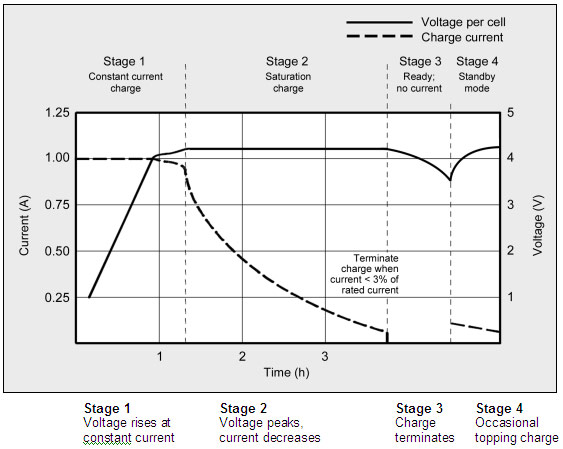
\includegraphics[width=0.5\textwidth]{images/2/2-1/cargaBateria.png}
    \caption{Ciclo de carga de una batería de ión de litio}
    \label{fig:2-1-cicloCarga}
\end{figure}

Si no se respeta el ciclo de carga de estas baterías, se tiene una alta probabilidad de que falle de forma violenta, siendo incluso un peligro de incendio. 

\subsubsection{Circuito de carga}

Para facilitarnos la tarea de respetar este ciclo hemos utilizado una solución integrada de Texas Instruments, el \texttt{BQ25606}, un cargador de una celda de litio que soporta hasta 3 amperios de corriente. \cite{BQ25606DataSheet}

Gracias a este circuito integrado y bastantes componentes externos, podemos diseñar un circuito que, a partir de una tensión de entrada entre 5 y 12 voltios y utilizando un convertidor reductor, carga la batería adecuadamente y de forma segura. 

La entrada al circuito puede ser a través de un conector \textit{Jack} de alimentación o un conector \textit{Micro USB}. Además, si se utiliza el segundo conector, el integrado se encarga de negociar el protocolo de carga rápida con la fuente de alimentación para incrementar la corriente de entrada y mejorar la potencia de carga. 

Además, si el circuito está conectado a la alimentación y la fuente tiene suficiente capacidad, la corriente de salida se obtiene de la entrada en lugar de la batería, gracias a la tecnología PowerPath de TI. Esta tecnología además permite balancear las tres corrientes, por lo que si el sistema requiriera de más corriente de la que la fuente de alimentación pudiera proveer, se obtendría también de la batería realizando un esfuerzo coordinado entre la fuente y la batería. Si por el contrario la fuente puede ofrecer más corriente de la que se está solicitando en la salida, se utiliza este excedente para cargar la batería.

Este circuito cuenta además con dos indicadores LED que informan sobre si la fuente de alimentación está conectada y las tensiones son correctas (verde en nuestro circuito) y si se está cargando la batería o hay algún fallo (roja en nuestro circuito). La segunda luz se mantiene encendida mientras se está cargando, se apaga cuando se ha finalizado la carga y parpadea a $1 Hz$ de frecuencia si hay algún error.

Para ofrecer todas estas características, el circuito integrado consta de una máquina de estados finitos y múltiples comparadores de error. Con esta inteligencia conmuta tres transistores para conectar la batería y para gestionar el convertidor conmutado síncrono que se construye. Se puede ver un diagrama de bloques resumido del circuito (obtenido de la hoja de catálogo) en la \autoref{fig:2-1-bloquesInternosBQ25606}

\begin{figure}[h]
    \centering
    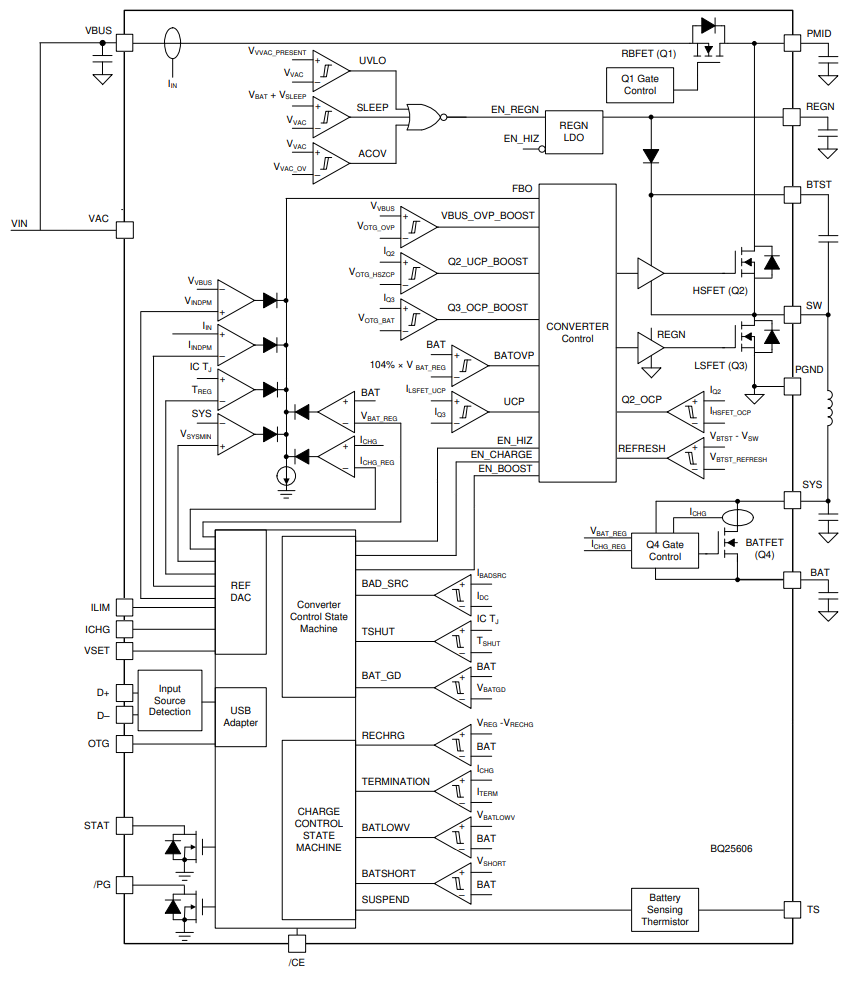
\includegraphics[width=0.5\textwidth]{images/2/2-1/BQ25606Bloques.png}
    \caption{Diagrama de bloques interno del BQ25606}
    \label{fig:2-1-bloquesInternosBQ25606}
\end{figure}

Este circuito ofrece a su salida una tensión aproximadamente igual a la de la batería durante el funcionamiento normal, por lo que está alrededor de los $3.7 V$. Sin embargo, si la tensión de la batería cae por debajo de $3.5 V$, el circuito se encarga de ofrecer dicha tensión a la salida, por lo que nunca bajará de dicho valor (mientras la batería puede ofrecer corriente y no esté descargada).

El circuito integrado ofrece también la posibilidad de utilizar una batería con sensor de temperatura integrado, pero no vamos a utilizarlo debido al incremento en coste de la misma.

En la hoja de catálogo del integrado se ofrece información sobre el proceso de diseño de un circuito alrededor de dicho integrado. Además, se tiene una nota de aplicación sobre el diseño de circuitos alrededor de este integrado \cite{texasinstrumentsDesigningStandaloneSingle}:

\begin{itemize}
    \item Inductancia de $2.2 \mu F$ para reducir el rizado de corriente.
    \item Pin \texttt{VSET} flotante para tensión de carga máxima de $4.208 V$.
    \item Divisor de tensión de dos resistencias de $10 k\Omega$ en \texttt{TS} para no utilizar divisor de tensión.
    \item Resistencia de $165 \Omega$ en \texttt{ILIM} para limitar la corriente de entrada cuando no se negocia carga rápida a $3 A$ (normalmente se utiliza mucho menos).
    \item Resistencia de $487 \Omega$ en \texttt{ICHG} para limitar la corriente de carga máxima a $1.4 A$ como se indica en las especificaciones de la batería.
    \item El resto de componentes se toman de la Figura 10-1 de la hoja de catálogo
\end{itemize}

Por tanto, esta parte del circuito queda como se puede ver en la \autoref{fig:circuito-carga-final}.

\begin{figure}[h]
    \centering
    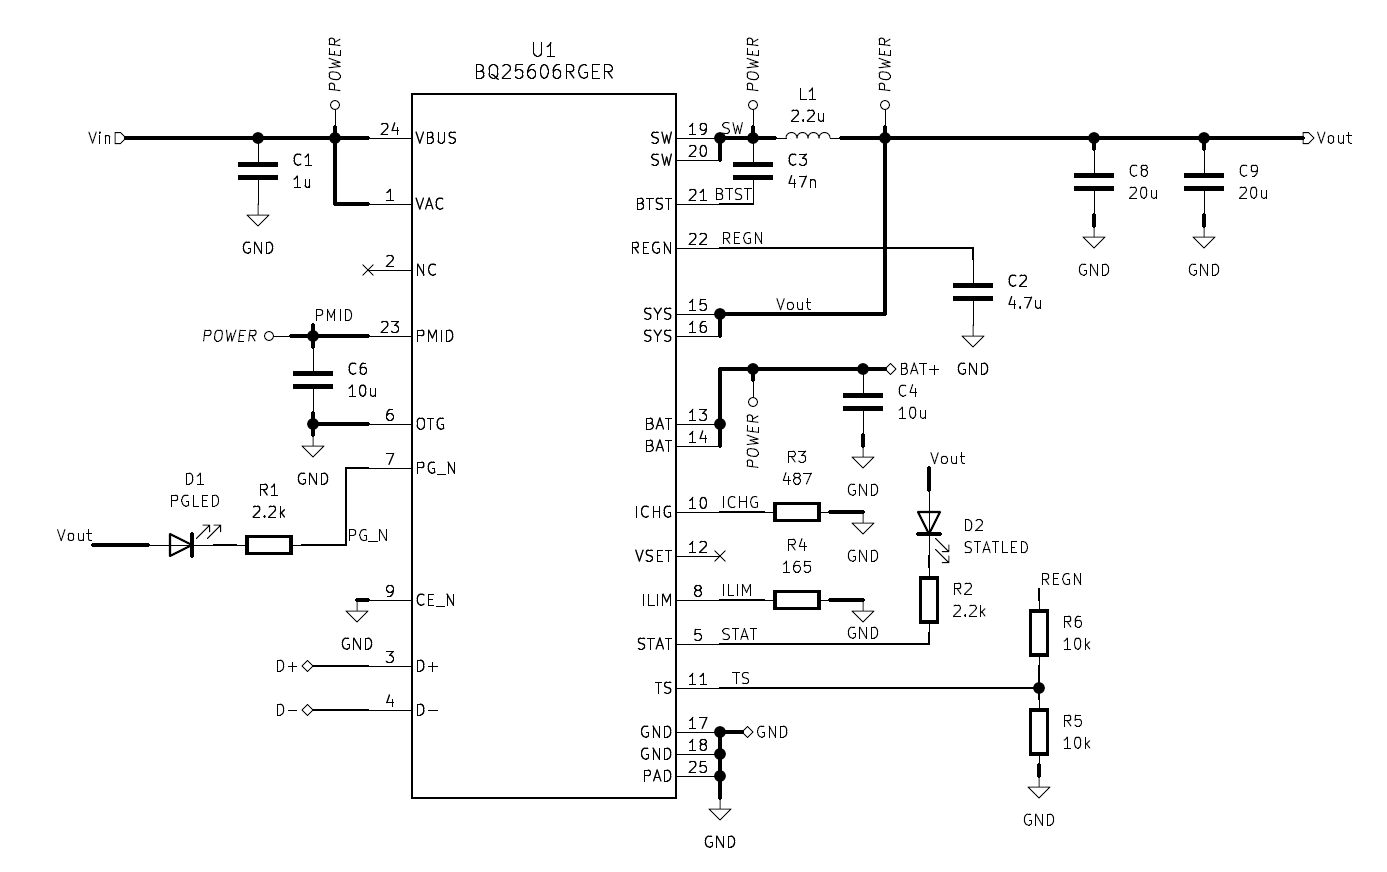
\includegraphics[width=\textwidth]{images/2/2-1/circuitoCarga.png}
    \caption{Subcircuito de carga de batería}
    \label{fig:circuito-carga-final}
\end{figure}

\subsubsection{Convertidor elevador}\label{subsubsec:convertidor_elevador}

La placa que utilizamos especifica una tensión de entrada de $7 V$ a $12 V$ si se utiliza el pin $V_{in}$ inferior. Preferimos utilizar este método ya que la entrada de $5 V$ no tiene protección y se puede dañar la placa si no se realiza todo el proceso adecuadamente.

Experimentalmente hemos notado que la placa utiliza la misma corriente de entrada para cualquier valor de tensión, por lo que seguramente utilice un convertidor de tensión lineal internamente para generar las tensiones. Por tanto, hemos preferido tomar el valor más pequeño de las tensiones de entrada para reducir la pérdida de potencia.

La tensión de salida del circuito de carga oscila entre los $3.5 V$ y los $4.2 V$, por lo que hemos diseñado un convertidor conmutado elevador o \textit{Boost Converter} para obtener dicha tensión a partir de la salida del cargador.

Un circuito convertidor elevador está compuesto básicamente por una bobina, un transistor y un controlador PWM.\ Como controlador PWM hemos utilizado otra solución integrada de Texas Instruments debido a la alta precisión que nos permite tener, ya que un fallo en este circuito podría dañar seriamente al resto del sistema. 

\subsubsection{Medidor de consumo}
\subsubsection{Diseño de PCB}